%\section{Event Reconstruction and Analysis} 

For each QE-like candidate, a muon and at least one proton are reconstructed as 
tracks, where the proton track originates from the most upstream position of 
the muon track. This selection includes all muons that exit either the side of the 
central tracking region or the downstream end. Therefore, the selection has
good acceptance for events with muon scattering angles up to 70$^{\circ}$ relative 
to the beam direction. Events are required to occur at least 22~cm from the edge 
of the scintillator and within the central 110~planes of the tracking region, defining a 
fiducial region of 5.57~metric tons. For $53\%$ of the events, the muon track 
is matched to a track in the \minos detector, allowing the charge and momentum to be 
determined. An additional $8\%$ of muons  
entering \minos are not tracked there. As for the muons that exit the 
\minerva outer calorimeter, only a lower-bound on the momentum is obtained. 
A minimum of five distinct energy depositions is required to form a 
proton track, resulting in a 110~MeV kinetic energy threshold. 
The proton tracks must stop in the inner region of \minerva. 

Particle identification (PID) and the reconstructed energy for
protons are determined using a track-based d$E/$d$x$ algorithm.
The algorithm fits the measured d$E/$d$x$ profile of 
a track to predicted profiles for both proton and pion hypotheses, 
and the two fit $\chi^2$ values are used to construct a proton PID consistency score~\cite{Twalton-thesis}. 
This fitting routine successfully identifies protons that
rescatter due to nuclear interactions and provides a kinetic energy
resolution of 5$\%$ for all identified protons. An event is retained 
if all non-muon tracks pass a cut on the proton PID consistency score.  

The remaining cuts are designed to remove inelastic background events with 
an untracked pion. Pions with kinetic energies above 100~MeV 
are likely to interact strongly within the detector materials, produce hadronic 
showers, and consequently are unable to be reconstructed as tracks. These events 
are removed by cutting on energy $E_{extra}$ that is not linked to a track and is located 
outside of a 10~cm sphere centered at the vertex. Excluding this vertex region 
when making this cut reduces sensitivity to mismodeling of low energy 
nucleons~\cite{Fields:2013zhk,Fiorentini:2013ezn}, which may arise from FSI or 
multinucleon effects.  Pions with kinetic energies below 100~MeV are removed 
using an algorithm that 
identifies Michel electrons from the $\pi \to \mu \to e$ decay chain occurring
near the vertex at a delayed time relative to the initial neutrino interaction.
After applying all cuts, the sample contains 40,102 QE-like candidates. 
The simulation predicts that 34.5\% of the events are from 
backgrounds containing at least one final-state pion, where the 
backgrounds are described below.

Measurement of the proton angle and momentum provides several variables 
that are sensitive to FSI. One variable is 
the angle~$\varphi$ between the $\nu$-muon and $\nu$-proton planes, and 
is shown in Fig.~\ref{fig:muon_proton_compare_angle} for both the data and 
two simulations: one with FSI and one without FSI. 
For both simulations, the non-QE-like 
background is tuned using a data-based procedure described below.
For QE scattering off a 
free neutron at rest $\varphi=180^\circ$. The detector resolution on 
$\varphi$ is 3.8~degrees, so the width shown on the distributions in 
Fig.~\ref{fig:muon_proton_compare_angle} is due to Fermi 
motion, inelastic scattering, and FSI effects. The comparison shows that \genie with 
FSI describes the data better than \genie without FSI. The remaining discrepancy 
suggests additional FSI or cross section effects not present in the \genie simulation.  

\begin{figure}[htpb]
\centering
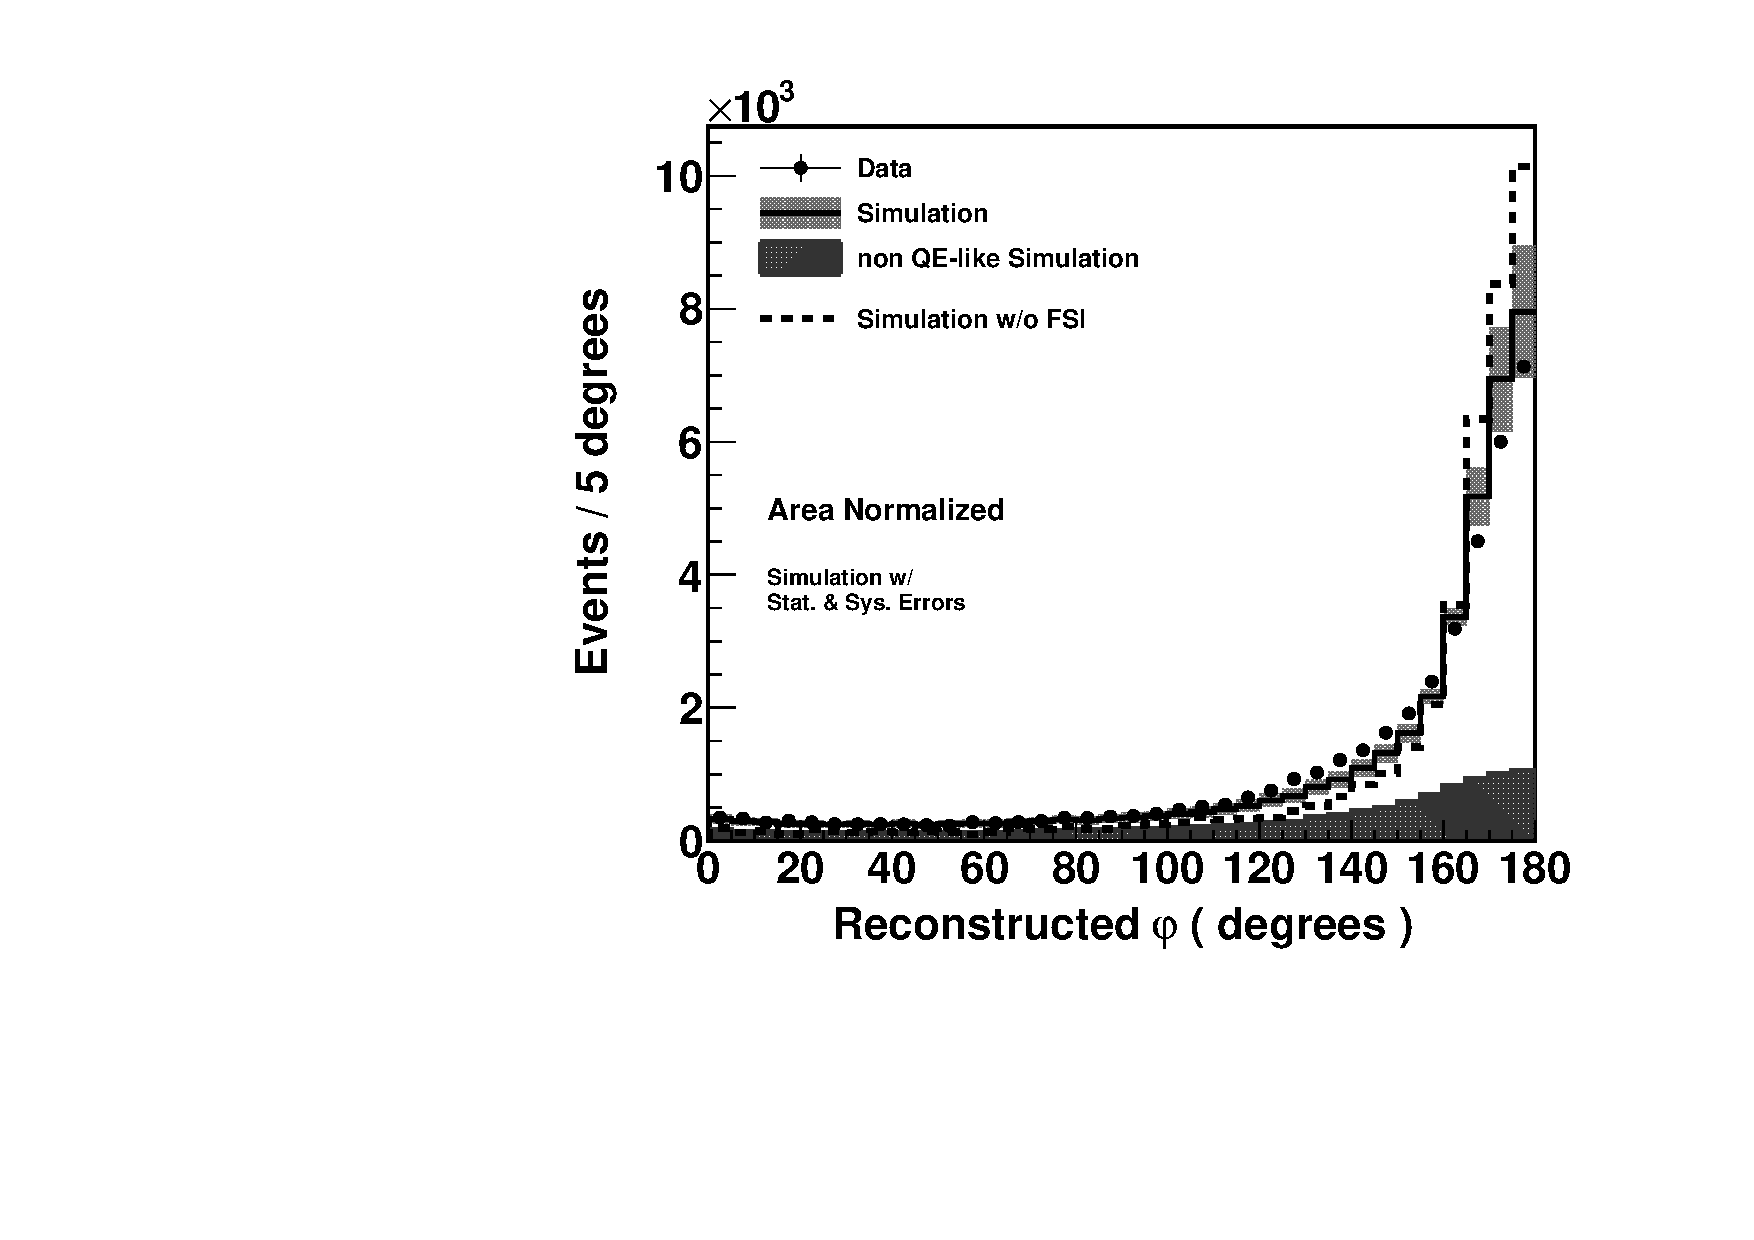
\includegraphics[width=\columnwidth]{figures/h_coplane_neutrino_genie_var_plastic_data_stats_area_tuned-bkgd.pdf}
\caption{Angle between the $\nu$-muon and $\nu$-proton planes for data (black points) and two
predictions from \genie, where the solid line prediction includes FSI
and the dashed line prediction does not. The total predictions have been normalized to the
data, and the non-QE-like predictions have been normalized to sidebands in the data.}
\label{fig:muon_proton_compare_angle}
\end{figure}

The differential cross section \dsdq is measured using the leading proton 
and the assumption of QE scattering from a neutron at rest. 
Under this assumption, \QSq is given by 
%%%%%%%%%%%%%%%%%%%%%%%%%%%%%%%%%%%%%%%%%%%%%%%%%%%%
\begin{equation*}
\QSqproton=(M_{n}-\epsilon_B)^2-M^2_{p}+2(M_{n}-\epsilon_{B})(T_{p}+M_{p}-M_{n}+\epsilon_{B}),
\end{equation*}
%%%%%%%%%%%%%%%%%%%%%%%%%%%%%%%%%%%%%%%%%%%%%%%%%%%%%
where $T_{p}$ is the kinetic energy of the proton, $M_{n,p}$ is the nucleon mass, 
and $\epsilon_B$ is the effective binding energy of +34 MeV~\cite{Moniz:1971mt}. 
This estimation of \QSqproton depends only on the $T_{p}$ of the leading proton.
%For QE scattering from a nucleon bound in a nucleus, 
This approximation of 
\QSqproton deviates from the \QSq estimated using only the muon. 
For the QE-like signal events that pass the analysis cuts, Fig.~\ref{fig:q2_correlation} 
shows \genie's  average values of various estimates of \QSq using truth information
as a function of \QSq as defined by the muon kinematics, namely: 
%%%%%%%%%%%%%%%%%%%%%%%%%%%%%%%%%%%%%%%%%%%%%%%%%%%%%%%%%%%%%%%%%%%%
\begin{equation*}
\QSqmuon=-m^{2}_{\mu}+2E_{\nu}(E_{\mu}-\sqrt{(E^{2}_{\mu}-m^{2}_{\mu})}\cos\theta_{\mu}),
\end{equation*}
%%%%%%%%%%%%%%%%%%%%%%%%%%%%%%%%%%%%%%%%%%%%%%%%%%%%%%%%%%%%%%%%%%%%
where $E_{\mu}$, $\theta_{\mu}$, and $m_{\mu}$ are the true energy, 
true scattering angle, and mass of the muon and $E_{\nu}$ is the true 
energy of the neutrino. The solid and short-dashed curves show \QSqmuon 
from the muon, and the discrepancy at \QSqmuon~$>$~1.7~GeV$^{2}$ is from
differences in the way the neutrino energy is estimated. The solid curve uses the 
neutrino's true energy, and short-dashed curve uses the QE hypothesis 
to estimate the neutrino energy using the muon's true energy and angle, which is given by 
%%%%%%%%%%%%%%%%%%%%%%%%%%%%%%%%%%%%%%%%%%%%%%%%%%%%%%%%%%
\begin{equation*}
E_{QE,\nu}=\frac{2(M_{n}-\epsilon_{B})E_{\mu}-[(M_{n}-\epsilon_{B})^{2}+m^{2}_{\mu}-M^{2}_{p}]}{2(M_{n}-\epsilon_{B}-E_{\mu}+\sqrt{(E^{2}_{\mu}-m^{2}_{\mu})}\cos\theta_{\mu})}.
\end{equation*}
%%%%%%%%%%%%%%%%%%%%%%%%%%%%%%%%%%%%%%%%%%%%%%%%%%%%%%%%%%
At higher \QSqmuon, the QE hypothesis inaccurately describes the inelastic 
component of the QE-like signal. 

The dotted and long-dashed curves show
\QSqproton from the proton, and the effects of FSI contribute to the discrepancy 
between the curves. The tracking threshold prevents the reconstruction of events 
with a leading proton having $T_{p}$~$<$~110~MeV, thereby resulting in a \QSqproton 
limit roughly 0.2~GeV$^{2}$ and poor acceptance for \QSqmuon~$<$~0.2~GeV$^{2}$.
Based on the Bodek-Ritchie~\cite{Bodek:1980ar,Bodek:1981wr} prescription,
\genie models the momentum distribution of initial-state nucleons by including a 
high-momentum tail extending beyond the Fermi momentum. Consequently at low \QSqmuon,
the analysis preferentially selects events where the initial-state 
nucleon momentum is greater than the Fermi momentum. This is a feature of the 
proton-based curves in Fig.~\ref{fig:q2_correlation}. 
The differences between the muon-based and proton-based estimates come from 
Fermi motion for the dotted curve and Fermi motion with FSI for the long-dashed curve, 
where such nuclear effects distort the shape of the \QSqproton distribution.

%%%%%%%%%%%%%%%%%%%%%%%%%%%%%%%%%%%%%%%%%%%%%%%%%%%%%%%%%%%%%%%%%%%%%%%%%%%%%%%%%%%%%%
\begin{figure}[htpb]
\centering
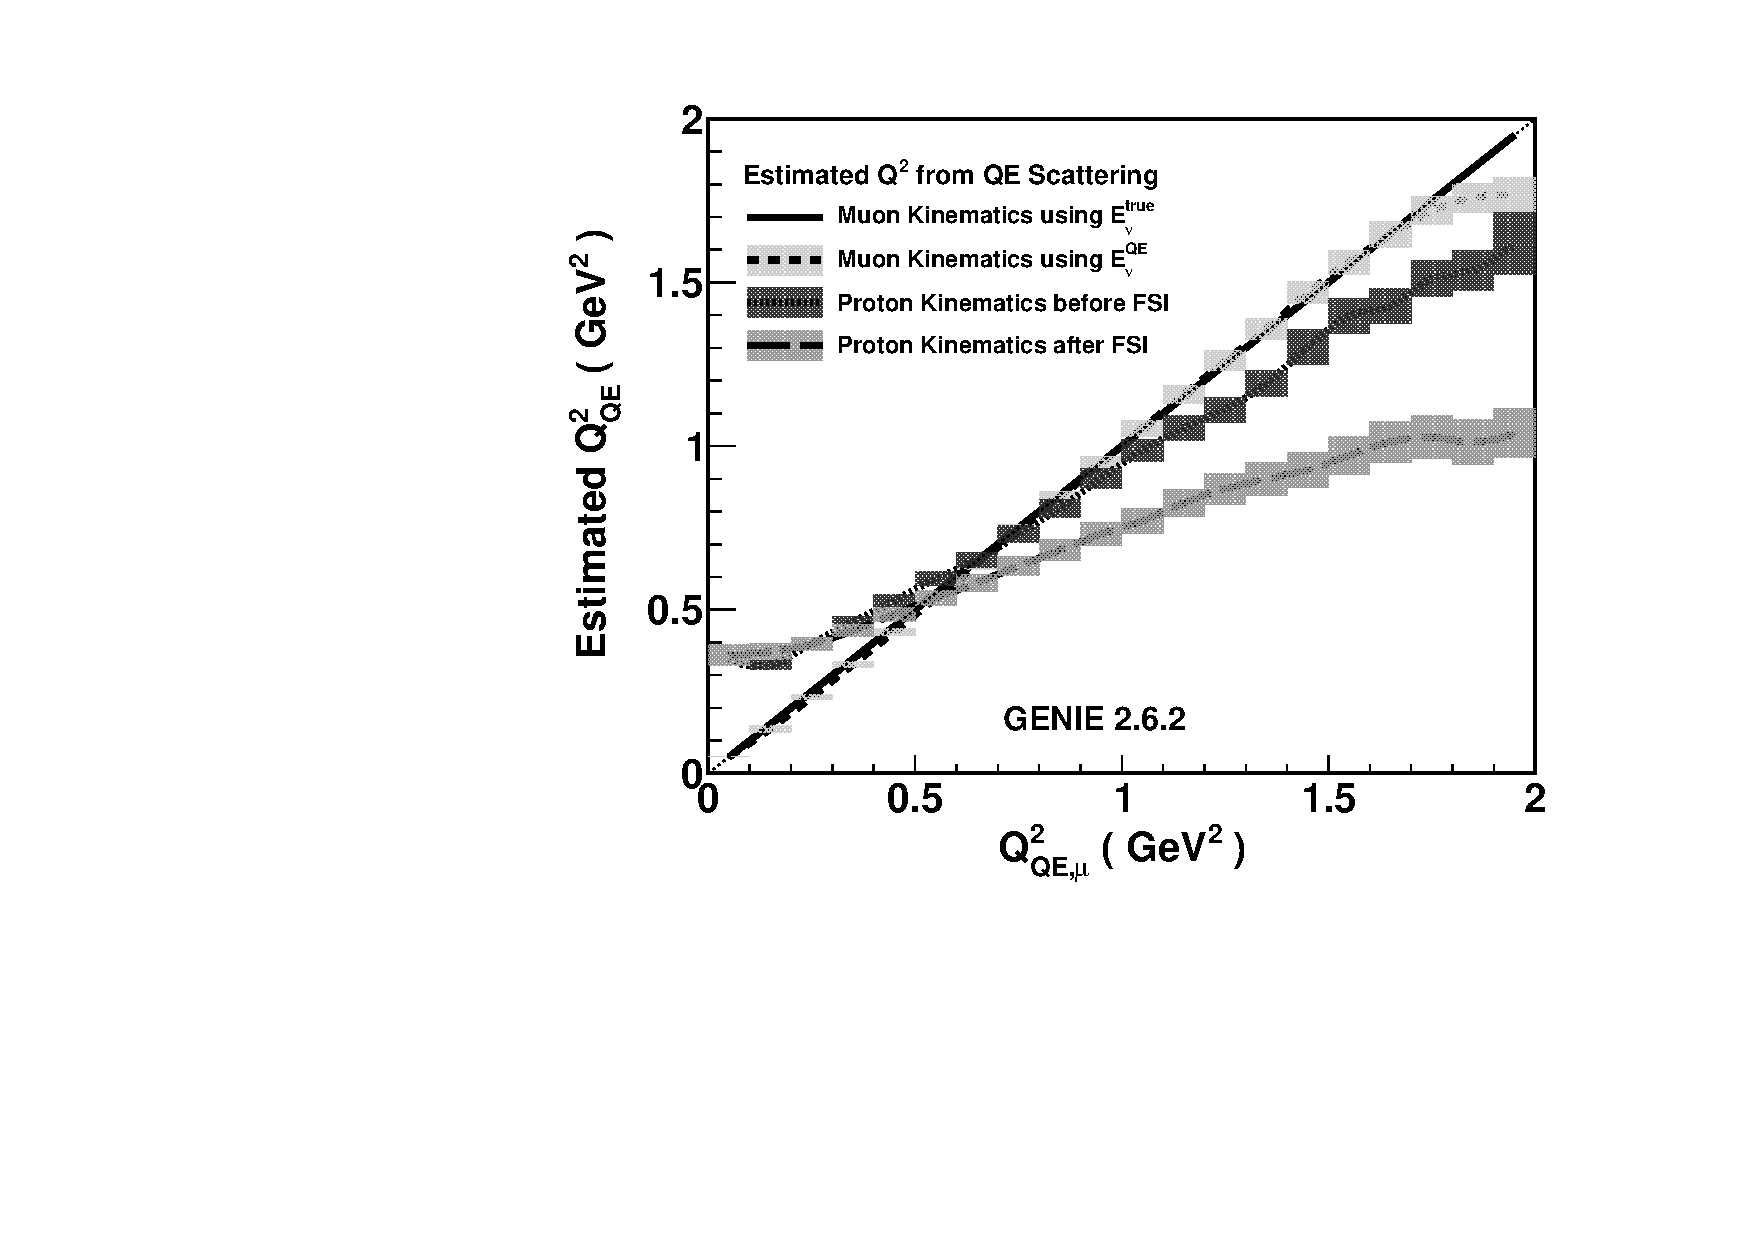
\includegraphics[width=\columnwidth]{figures/h_event_proton_plastic_mc_CV_WithStatErr_num_profile_overlay3.pdf}
\caption{Comparisons between several \QSq estimates as function of the \QSq estimated
using muon kinematics for the QE-like signal events that pass the reconstruction
and analysis cuts, as described in the text. The error bands include 
statistical and \genie systematic uncertainties.}
\label{fig:q2_correlation}
\end{figure}
%%%%%%%%%%%%%%%%%%%%%%%%%%%%%%%%%%%%%%%%%%%%%%%%%%%%%%%%%%%%%%%%%%%%%%%%%%%%%%%%%%%%%%%%

The reconstructed \QSqproton distribution is shown in Fig.~\ref{fig:ccqelike_reco_q2_pot}. 
The data are compared to \genie predictions of the QE-like signal and 
backgrounds, where the background estimates have been tuned using the data.
The largest background comes from baryon resonance 
production, predominantly $\Delta(1232)$. A smaller background originates
from non-resonant inelastic pion production, which is referred to as
deep-inelastic scattering (DIS) in \genie.
In the tuning procedure, the non-QE-like backgrounds are categorized 
as one of two processes: ``resonant'' or ``DIS plus other'' (hereafter denoted DIS+), 
where the ``other'' includes $\overline{\nu}_{\mu}$ interactions
and a smaller neutral current component. Four distinct sideband regions of the 
$E_{extra}$ distribution are used to extract normalization constants for each process. 
The sidebands further from the signal region are predicted to contain a larger estimated fraction 
of DIS+ relative to the resonant fraction and are more consistent with the data. 
By separating the simulated backgrounds into two processes, 
the backgrounds in each \QSqproton bin are determined from a 
linear fit that simultaneously matches the simulated background to data 
in all sideband regions. The tuning results indicate that 
the baryon resonance production background should be reduced by roughly 50$\%$. 
The DIS+ background prediction remains nearly unchanged for \QSqproton~$>$~0.5~GeV$^{2}$ 
and increases by 20$-$60$\%$ in \QSqproton regions between 0.15 to 0.5~GeV$^{2}$.

%%%%%%%%%%%%%%%%%%%%%%%%%%%%%%%%%%%%%%%%%%%%%%%%%%%%%%%%%%%%%%%
\begin{figure}[tp]
\centering
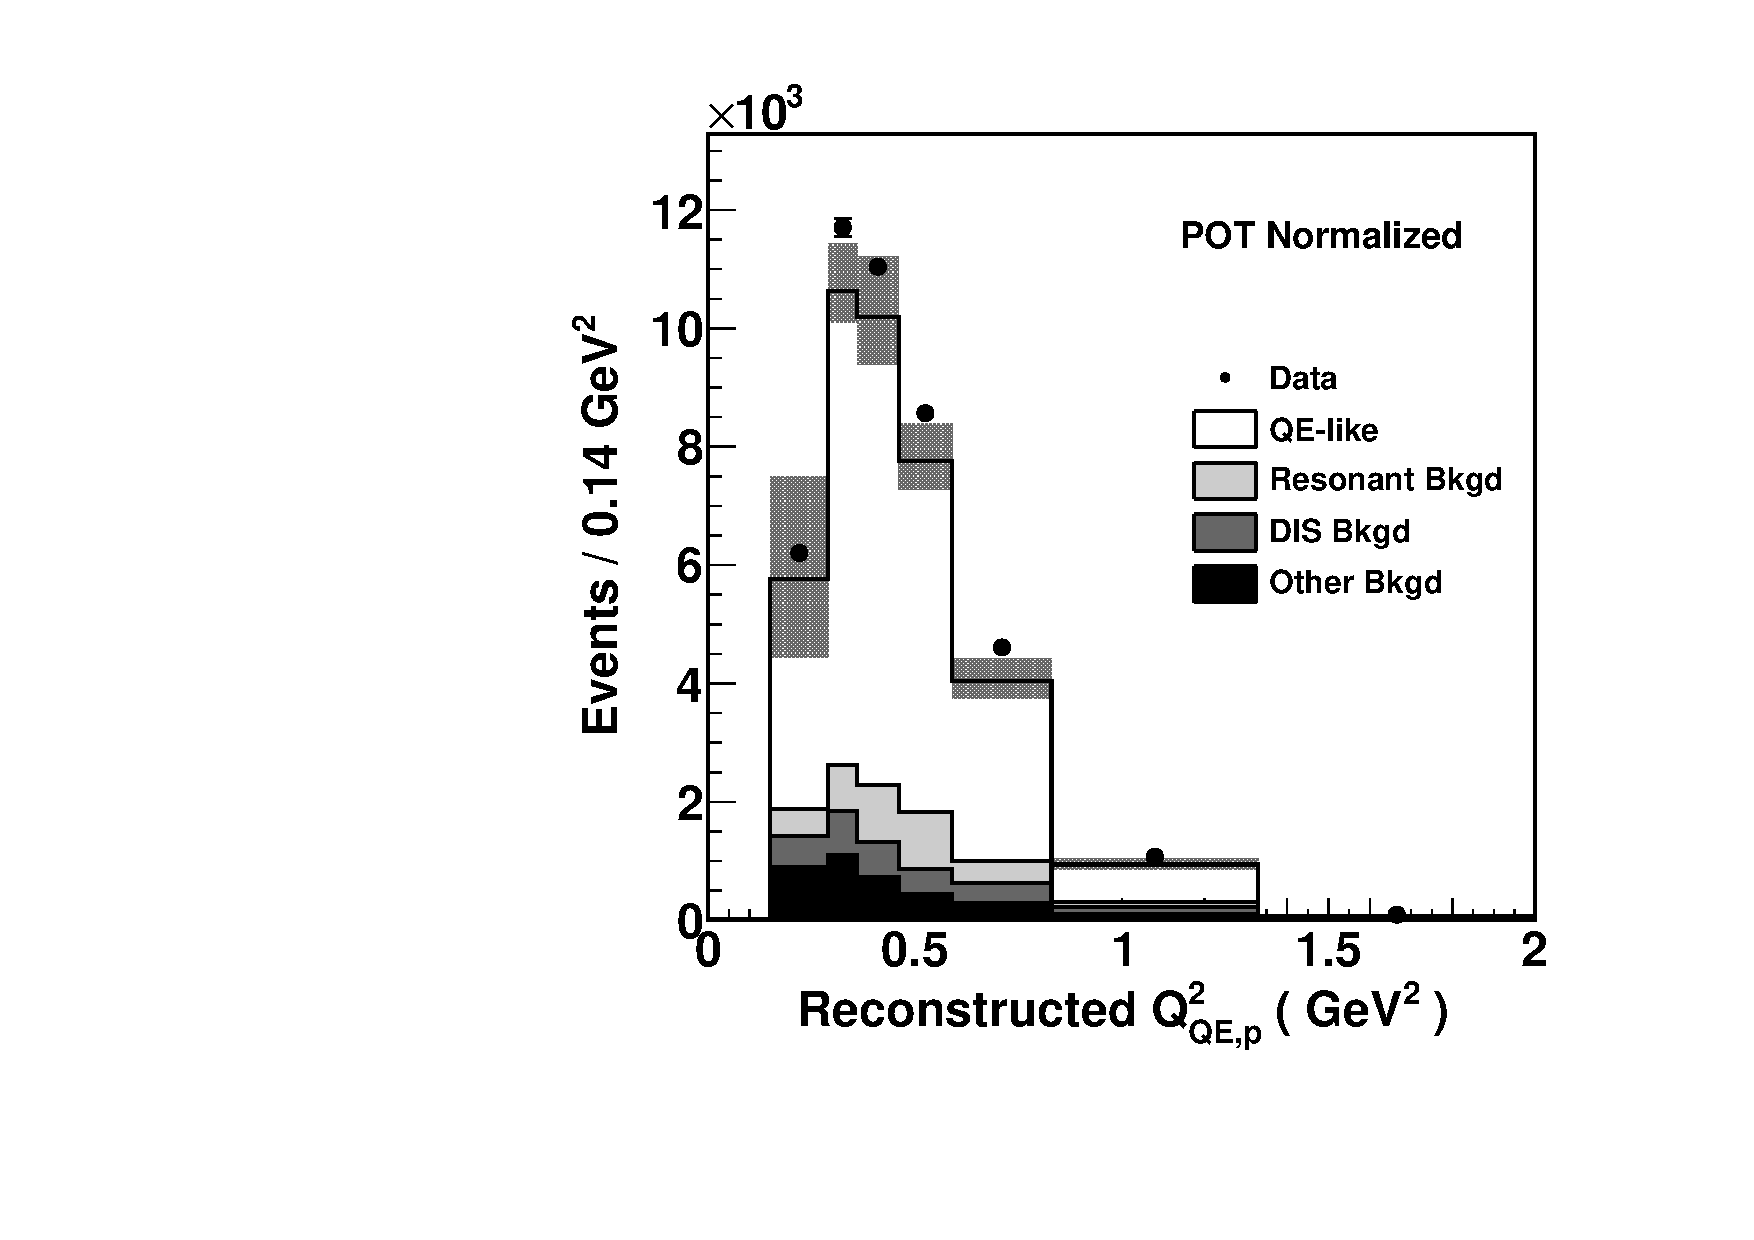
\includegraphics[width=\columnwidth]{figures/h_proton_q2_constrain_phys_bkgd_neutrino_genie_var_plastic_data_stack5_pot.pdf}
\caption{Distribution of $Q^2$ of the QE-like events determined by the leading proton 
track reconstruction in data and simulation, where the background estimates are 
tuned to sideband samples of the data. }
\label{fig:ccqelike_reco_q2_pot}
\end{figure}
%%%%%%%%%%%%%%%%%%%%%%%%%%%%%%%%%%%%%%%%

After subtracting the data-tuned backgrounds, the yield is corrected for detector 
smearing of the leading proton energy via a Bayesian unfolding procedure using four 
iterations~\cite{D'Agostini:1994zf}. The simulation is used to correct for geometric 
acceptance and efficiency for the unfolded distribution. To obtain the flux-averaged 
differential cross section, the yields are divided by the number of nucleons in the 
fiducial volume (3.294~$\times$~$10^{30}$) and the integrated \numu  
flux below 100~GeV (3.286~$\times$~$10^{-8}\rm /cm^{2}/POT$).

